\documentclass[aspectratio=169,12pt]{beamer}
\usepackage[utf8]{inputenc}
\usepackage[T2A]{fontenc}
\usepackage[russian]{babel}
\usepackage{graphicx}
\usepackage{booktabs}
\usepackage{hyperref}

% Минималистичная светлая тема
\usetheme{default}
\usecolortheme{dove}

% Приятный синий акцент
\definecolor{accent}{RGB}{0, 102, 204}
\definecolor{lightgray}{RGB}{245, 245, 245}

\setbeamercolor{frametitle}{fg=accent, bg=white}
\setbeamercolor{title}{fg=accent}
\setbeamercolor{structure}{fg=accent}
\setbeamercolor{itemize item}{fg=accent}
\setbeamercolor{itemize subitem}{fg=accent!70}
\setbeamercolor{block title}{bg=accent, fg=white}
\setbeamercolor{block body}{bg=lightgray}

\setbeamertemplate{navigation symbols}{}
\setbeamertemplate{footline}[frame number]
\setbeamertemplate{itemize items}[circle]
\setbeamerfont{frametitle}{size=\Large, series=\bfseries}

% Метаданные
\title{RAG Чат-бот по роману\\«Мастер и Маргарита»}
\subtitle{Курс «Введение в LLM»}
\author{Команда bookworm}
\institute{ИТМО}
\date{Январь 2026}

\begin{document}

% ========== ТИТУЛЬНЫЙ СЛАЙД ==========
\begin{frame}
\titlepage
\vspace{-1em}
\centering
\small Горбунов Дмитрий, Ковалева Дарина, Тельнов Федор, Мацаков Борис
\end{frame}

% ========== ПРОБЛЕМА ==========
\begin{frame}{Проблема и цели проекта}

\textbf{Проблема:}
\begin{itemize}
    \item «Мастер и Маргарита» - много персонажей и сюжетных линий
    \item Поиск информации требует перечитывания книги
    \item LLM без RAG галлюцинирует и путает детали сюжета
\end{itemize}

\vspace{1em}
\textbf{Цель:} Создать чат-бота, который отвечает на вопросы \textbf{только на основе текста книги}

\vspace{1em}
\textbf{Задачи:}
\begin{enumerate}
    \item Подготовить текст для RAG-поиска
    \item Реализовать retrieval-пайплайн
    \item Создать удобный веб-интерфейс
    \item Оценить качество ответов
\end{enumerate}

\end{frame}

% ========== СБОР ДАННЫХ ==========
\begin{frame}{Сбор и подготовка данных}

\begin{columns}
\begin{column}{0.5\textwidth}
\textbf{Источник:}
\begin{itemize}
    \item Флибуста (FB2 формат)
    \item ~580 000 символов
    \item 32 главы + эпилог
\end{itemize}

\vspace{1em}
\textbf{Подготовка:}
\begin{enumerate}
    \item Парсинг FB2 (XML)
    \item Разбиение на главы
    \item Chunking: 800 симв., overlap 100
    \item Эмбеддинги: GigaChat (1024 dim)
    \item Индексация: FAISS
\end{enumerate}
\end{column}

\begin{column}{0.5\textwidth}
\textbf{Итог:}
\begin{table}
\centering
\begin{tabular}{ll}
\toprule
Метрика & Значение \\
\midrule
Чанков & 1 182 \\
Размерность & 1024 \\
Индекс & FAISS FlatIP \\
\bottomrule
\end{tabular}
\end{table}

\vspace{1em}
\textbf{Хранение:}
\begin{itemize}
    \item chunks.parquet
    \item embeddings.parquet
    \item faiss\_index/
\end{itemize}
\end{column}
\end{columns}

\end{frame}

% ========== АРХИТЕКТУРА ==========
\begin{frame}{Архитектура решения}

\begin{center}
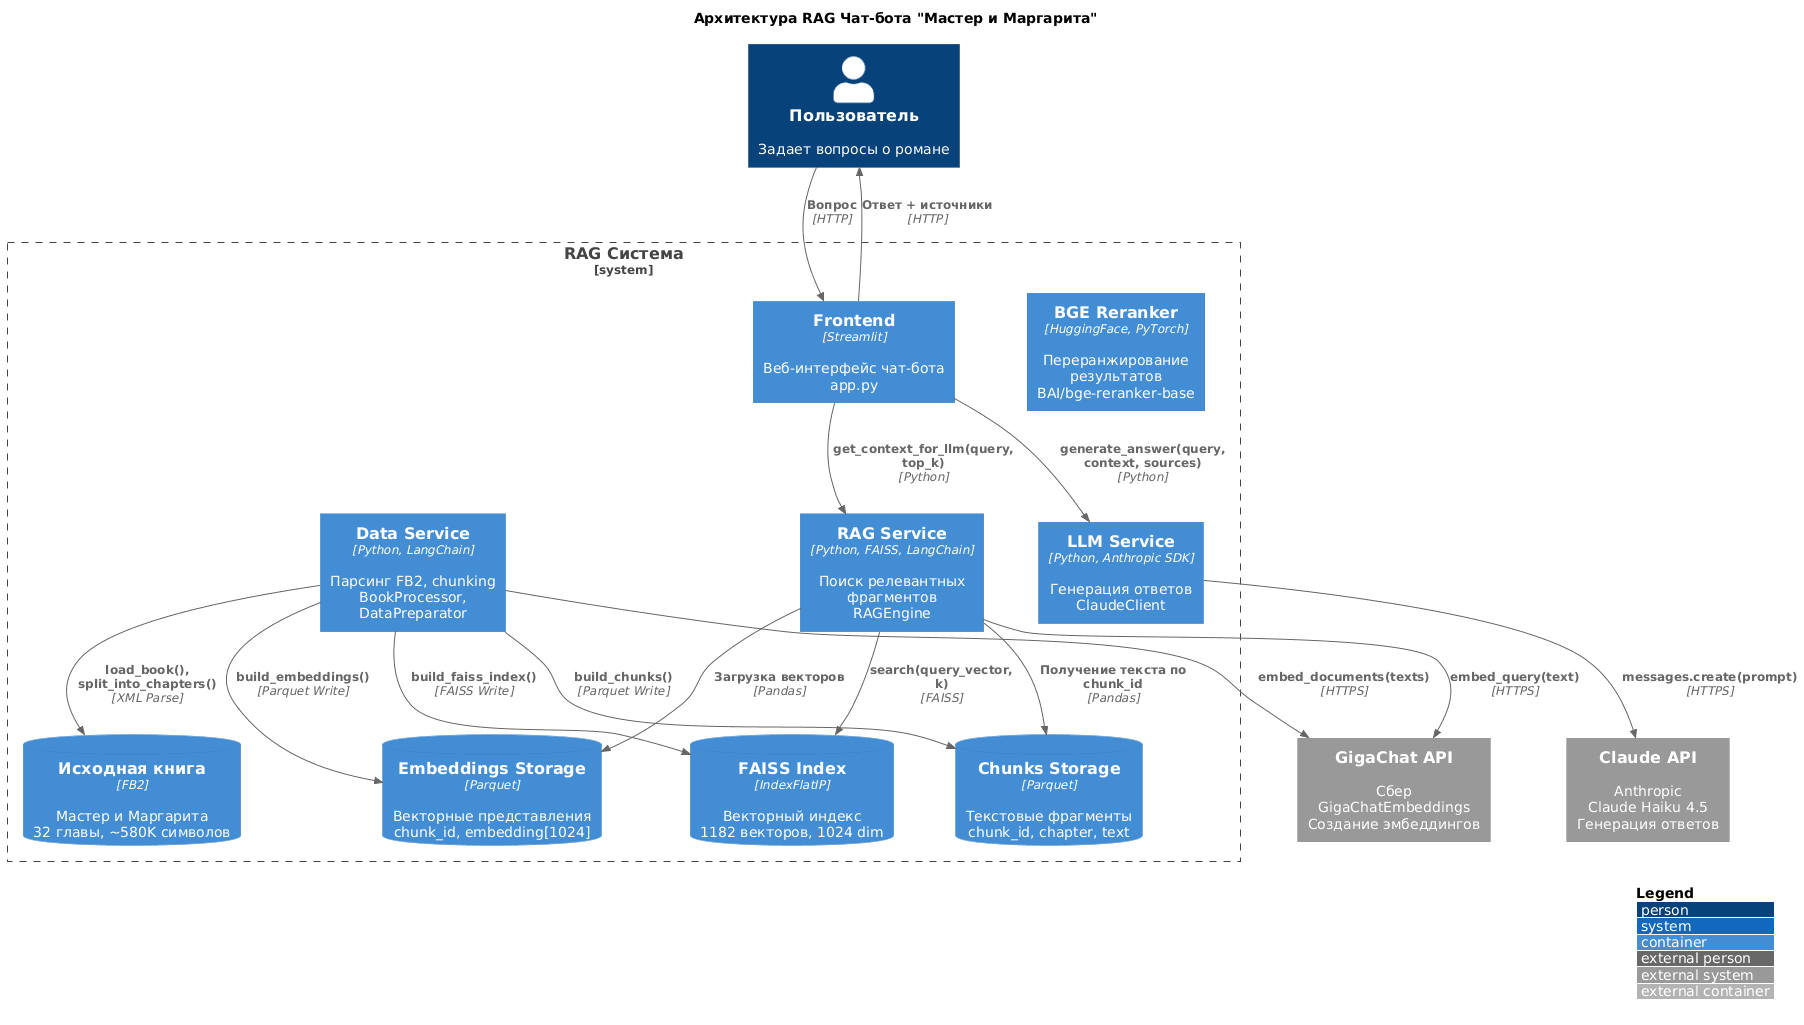
\includegraphics[width=0.85\textwidth]{architecture.png}
\end{center}

\end{frame}

% ========== КОМПОНЕНТЫ ==========
\begin{frame}{Компоненты системы}

\begin{columns}
\begin{column}{0.5\textwidth}
\textbf{Data Service:}
\begin{itemize}
    \item Парсинг FB2
    \item RecursiveCharacterTextSplitter
    \item Метаданные глав
\end{itemize}

\vspace{0.5em}
\textbf{RAG Service:}
\begin{itemize}
    \item GigaChat Embeddings
    \item FAISS IndexFlatIP
    \item BGE-reranker-base (опц.)
\end{itemize}
\end{column}

\begin{column}{0.5\textwidth}
\textbf{LLM Service:}
\begin{itemize}
    \item OpenRouter (GPT-4o-mini)
    \item Claude Haiku (альт.)
    \item Строгий промпт: только контекст
\end{itemize}

\vspace{0.5em}
\textbf{Frontend:}
\begin{itemize}
    \item Streamlit
    \item История чата
    \item Показ источников
    \item Переключатель реранкера
\end{itemize}
\end{column}
\end{columns}

\end{frame}

% ========== ОЦЕНКА КАЧЕСТВА ==========
\begin{frame}{Оценка качества}

\textbf{Инструмент:} RAGAS (Retrieval Augmented Generation Assessment)

\vspace{0.5em}
\textbf{Валидационная выборка:} 70 вопросов с эталонными ответами

\vspace{1em}
\begin{table}
\centering
\begin{tabular}{lp{7cm}}
\toprule
\textbf{Метрика} & \textbf{Что измеряет} \\
\midrule
Faithfulness & Нет галлюцинаций в ответе \\
Answer Relevancy & Релевантность ответа вопросу \\
Context Precision & Точность найденных фрагментов \\
Context Recall & Полнота покрытия эталонного ответа \\
\bottomrule
\end{tabular}
\end{table}

\end{frame}

% ========== ЭКСПЕРИМЕНТЫ ==========
\begin{frame}{Эксперименты и результаты}

\begin{columns}
\begin{column}{0.55\textwidth}
\textbf{Финальные метрики (70 вопросов):}

\begin{table}
\centering
\begin{tabular}{lcc}
\toprule
Метрика & Без реранк. & С реранк. \\
\midrule
Faithfulness & \textbf{0.856} & 0.821 \\
Answer Relevancy & 0.358 & \textbf{0.398} \\
Context Precision & \textbf{0.487} & 0.474 \\
Context Recall & \textbf{0.431} & 0.421 \\
\bottomrule
\end{tabular}
\end{table}
\end{column}

\begin{column}{0.45\textwidth}
\textbf{Выводы:}
\begin{itemize}
    \item Реранкер: +0.040 к relevancy
    \item GigaChat эмбеддинги уже хорошо ранжируют
    \item Faithfulness 0.856 - мало галлюцинаций
\end{itemize}

\vspace{0.5em}
\textbf{Что не работало:}
\begin{itemize}
    \item OpenAI Embeddings - VPN
    \item GigaChat LLM - rate limits
\end{itemize}
\end{column}
\end{columns}

\end{frame}

% ========== ПРОДУКТ ==========
\begin{frame}{Итоговый продукт}

\textbf{Возможности:}
\begin{itemize}
    \item Ответы на вопросы по книге
    \item Показ источников и цитат
    \item Переключение реранкера
    \item История диалога
\end{itemize}

\vspace{1em}
\textbf{Запуск:}
\begin{itemize}
    \item \texttt{pip install -r requirements.txt}
    \item \texttt{streamlit run frontend/app.py}
    \item Или: \texttt{docker-compose up}
\end{itemize}

\end{frame}

% ========== ИНТЕРФЕЙС ==========
\begin{frame}{Интерфейс}

\begin{center}
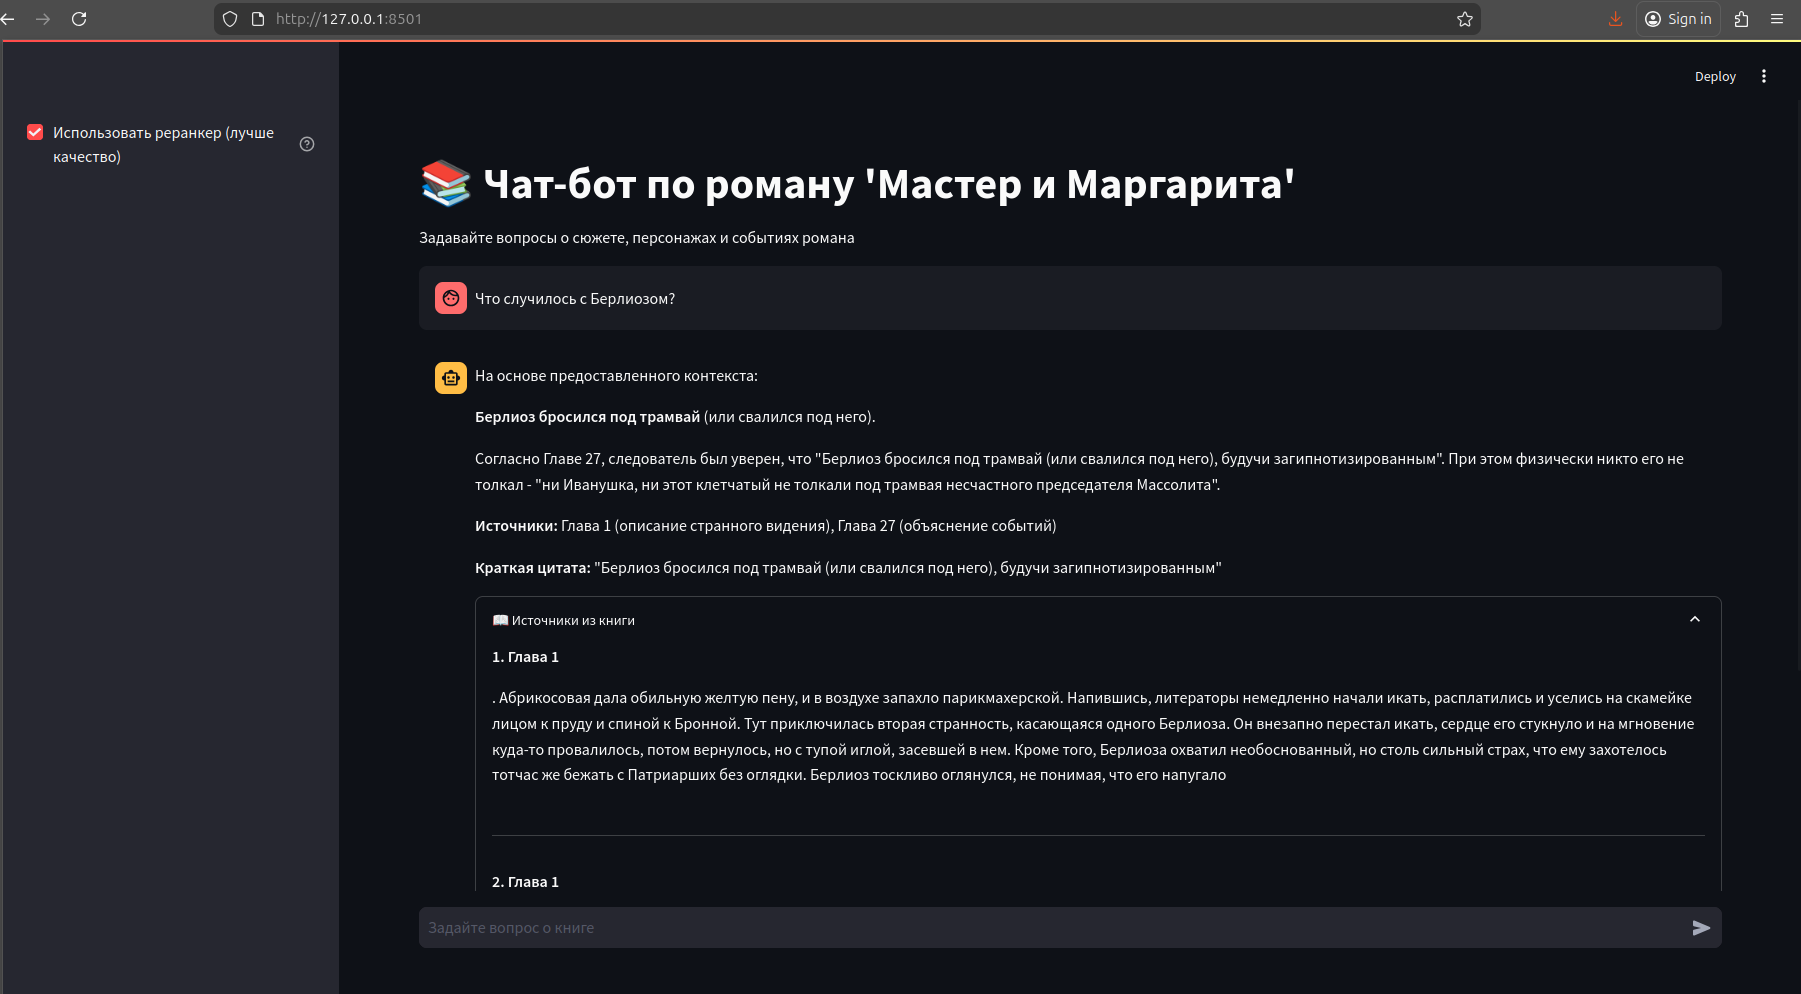
\includegraphics[width=0.85\textwidth]{main_screen.png}
\end{center}

\end{frame}

% ========== КОМАНДА ==========
\begin{frame}{Команда и распределение ролей}

\begin{table}
\centering
\begin{tabular}{ll}
\toprule
\textbf{Участник} & \textbf{Вклад} \\
\midrule
Горбунов Дмитрий & MVP: chunking, embeddings, RAG-пайплайн, UI \\
Ковалева Дарина & Реранкер (BGE), сравнительный анализ \\
Тельнов Федор & Проектирование архитектуры, диаграммы \\
Мацаков Борис & Модуль оценки (RAGAS), валидация качества \\
\bottomrule
\end{tabular}
\end{table}

\vspace{1em}
\centering
\textbf{Репозиторий:} \url{https://github.com/bookworm-itmo/llm-intro-project}

\end{frame}

% ========== ВОПРОСЫ ==========
\begin{frame}
\centering
\Huge Вопросы?

\vspace{2em}
\normalsize
\textbf{GitHub:} \url{https://github.com/bookworm-itmo/llm-intro-project}

\vspace{1em}
\textbf{Telegram:} @grbn\_dima
\end{frame}

\end{document}
